\section{Implementation and Evaluation}
\label{sec:fingerprint-implementation}

In order to facilitate easy implementation in a wide range of languages, including those from the functional programming paradigm, the operations of the fingerprint summary are presented in the pseudocode as free-standing functions without side effects.
The Java implementation takes full advantage of the object-oriented programming paradigm, however, and the corresponding methods are instance members of the mutable \lstinline{Fingerprint} class, which implements the \lstinline{getHashValue()} query method of the \lstinline{IdentificationSummary} interface.
The class also overrides \lstinline{Object.equals(Object)} and, therefore, \lstinline{Object.hashCode()} in order to implement the equality operation.
Since it is assumed that the largest item in a stream cannot be known beforehand, the universe of items used in the implementation is defined to be a non-negative subset of the ubiquitous \num{32}~bit signed \lstinline{int} data type.
As a result, an unchecked \lstinline{IllegalArgumentException} is raised if a negative item is passed to the \lstinline{update(int, int)} method.
The fixed superset of the universe allows the prime number to be embedded directly in the implementation.
Since this determines the greatest possible value of the base, which is at most squared during the update operation, the greatest exact primitive value that can be used is the greatest prime less than the square root of the upper bound \( 2^{63} - 1 \) of the \num{64}~bit \lstinline{long} data type, which is \num{3037000493}.
The exponentiation by squaring method is implemented as a static method in the \lstinline{Math} utility class.

The \lstinline{FingerprintAccumulator} class adapts the summary for use in Apache Spark (see \cref{subsec:introduction-structure-library}).
This allowed two types of test to be performed on the implementation of the fingerprint summary.
The first was a test of the accuracy of its query and equality operations.
The second was a test of the relationship between the size of a dataset and the time taken to construct its summary.
All tests were performed on a single machine using an Intel Core i5-9300H CPU with a base clock speed of \SI{2.40}{\giga\hertz}, four physical cores and eight logical processors, and \SI{8}{\gibi\byte} of RAM\@.
For information regarding how to run the tests, see \cref{app:repository}.

A failure in the accuracy of the fingerprint summary equality operation occurs when the fingerprint summaries of two different multisets have the same hash value.
This is a false positive.
An upper bound on the probability of such a failure is determined by the ratio of the size \( u - 1 \) of the positive subset of the universe from which items are drawn to the size \( p - 1 \) of the interval from which the base \( \alpha \) is drawn (see \cref{subsec:fingerprint-analysis-accuracy}).
Since the implementation uses the fixed prime number \num{3037000493}, this failure bound can be verified empirically by varying the upper bound \( u - 1 \) of the universe.

Five series of accuracy tests were performed using the upper bounds \( 2^{8} - 1 \), \( 2^{12} - 1 \), \( 2^{16} - 1 \), \( 2^{20} - 1 \) and~\( 2^{24} - 1 \).
A fixed lower bound of zero was used in all tests.
This is the least value a fingerprint summary can accept.
To obtain a representative sample of results, each test was run \num{25}~times.
On each run, an artificial dataset was generated by drawing pairs of items and weights uniformly at random from the universe of items and the interval of weights, respectively.
Each entry in the dataset was itself a pair of these item--weight pairs, meaning that the dataset represented two multisets of the same size.
A total of \( 2^{16} \) such \emph{pairs of pairs} were drawn for each dataset.
This dataset size was chosen as it is large enough to warrant the use of a streaming algorithm, which offers a reduction in space requirements in exchange for less accurate results.
Conversely, it is not so large that the time and space consumed by the test could prevent other tests from being performed.
A larger dataset would be of no benefit, as the accuracy of a fingerprint summary is independent of the size of the data it summarizes.
Since the accuracy is also independent of the interval from which weights are drawn, the weights were drawn from a smaller interval \( \dataintegerinterval{-2^{7}, 2^{7} - 1} \) as this would not consume much space in the dataset, which was stored as a comma-delimited text file.

Using the Apache~Spark stream processing framework, each dataset was read as input and passed one pair at a time to three \lstinline{FingerprintAccumulator} objects.
These constructed a \lstinline{Fingerprint} of the first multiset, another of the first multiset read in reverse order, and one more of the second multiset, respectively.
Apache~Spark was run using one worker thread for each of the eight logical processors of the test machine.
By running the summary construction in parallel, the correctness of the merge operation was also verified.
Since streaming algorithms use commutative update operations and are designed to handle streams of arbitrary order, the first and second of these \lstinline{Fingerprint} objects should hold the same hash value, since they summarize the same multiset.
This equality check verifies that the update and merge operations are indeed commutative.
The first and third of the \lstinline{Fingerprint} objects should hold different hash values with probability at least \( 1 - \delta \), where \( \delta \) is given by \cref{eq:fingerprint-implementation-accuracy-upper-bound}, unless the two randomly generated multisets are equal.
Over all of the runs that used a universe of a given size, this inequality check verified the corresponding upper bound on the probability of a false positive.
A test is considered to have passed if both of these checks passed.

\begin{equation}
  \label{eq:fingerprint-implementation-accuracy-upper-bound}
  \delta = \frac{u - 1}{p - 1}
\end{equation}

\begin{table}
  \centering
  \caption{Results of the accuracy tests}
  \label{tab:fingerprint-implementation-accuracy}
  \begin{tabular}{
  S[
    table-alignment = right,
    table-format = 2,
  ]
  S[
    round-mode = figures,
    round-precision = 3,
    table-alignment = right,
    table-format = 1.2e-1,
  ]
  S[
    table-alignment = right,
    table-format = 1,
  ]
}
  \toprule
  {Rows} & \multicolumn{2}{c}{Failure proportion} \\
  \cmidrule{2-3}
  & {Upper bound} & {Observation} \\
  \midrule
  3 & 0.04978706837 & 0 \\
  5 & 6.737946999e-3 & 0 \\
  7 & 9.118819656e-4 & 0 \\
  9 & 1.234098041e-4 & 0 \\
  11 & 1.670170079e-5 & 0 \\
  \bottomrule
\end{tabular}
%
\end{table}

The results of all \num{25}~runs of each of the five accuracy tests are presented in \cref{tab:fingerprint-implementation-accuracy}.
This includes the item upper bound, the upper bound on the probability of a false positive, and the proportion of failures observed.
Both the equality check and the inequality check passed on every run of every test.
This provides an empirical verification of the correctness of both the design of the fingerprint summary, and the upper bound on the probability of a false positive.
It should be noted that the failure bound of the first test corresponds to odds of approximately one in \num{12}~million.
Therefore, a more reliable verification could have been obtained by performing a minimum of \num{12}~million runs, each using a different base.
An even more precise verification could have been achieved by constructing one summary of a particular dataset for each of the \num{3037000492} possible values of the base.
Of course, this scale of testing was deemed both infeasible and unnecessary.
The total of \num{125}~runs was sufficient to show that the probability of a failure is low, even for a high item upper bound of \( 2^{24} \).

The relationship between the size of a dataset and the time taken to construct its summary was tested via performance tests.
Five series of performance tests were performed using dataset sizes of \( 2^{8} \), \( 2^{12} \), \( 2^{16} \), \( 2^{20} \) and~\( 2^{24} \).
For each of the five series, \num{26}~artificial datasets were generated by drawing the corresponding numbers of pairs of items and weights, in the same manner as for the accuracy tests.
Since only the size of the data was varied for these tests, the items were drawn from the non-negative subset of the full range of the \num{32}-bit signed integer data type, and the weights were drawn from the arbitrary fixed interval \( \dataintegerinterval{-2^{7}, 2^{7} - 1} \).
After all \num{26}~datasets had been generated, the construction of the \lstinline{Fingerprint} of each dataset was timed using only a single worker thread.
The execution time was calculated as the positive difference between the values returned by calls to \lstinline{System.nanoTime()} immediately before and immediately after the construction.
Although this method gives nanosecond precision by querying the most precise available system timer~\citep{o14}, it does not necessarily give nanosecond accuracy, since there is no guarantee regarding the frequency with which this value is updated~\citep{lambert08}.
Nevertheless, it can be assumed that, on average, it is accurate to within hundreds of nanoseconds~\citep{kuperberg09}.
The first run of each series of tests was discarded, as this run `warms up' the test architecture by loading process data into memory and, therefore, encounters page faults and cache misses that should not be considered a feature of normal operation~\citep{luo04}.
The median of the remaining \num{25}~runs was calculated.
Since the execution time can vary greatly due to the presence of other processes, the median is more suitable than the mean as a representation of the typical execution time, as it is not so easily skewed by outliers, and remains meaningful after normalization~\citep{fleming86}.
A sixth series of tests was performed using a dataset containing only a single item--weight pair.
The median execution time of this series was taken as an approximation of the fixed overhead associated with starting the test and initializing the summary.
This was subtracted from the median execution times of the other series of tests in order to normalize them such that they represent only the time taken to update the summary for each item--weight pair in the corresponding dataset.

\begin{table}
  \centering
  \caption{Results of the performance tests}
  \label{tab:fingerprint-implementation-performance}
  \begin{tabular}{
  S[
    table-alignment = right,
    table-format = 8,
  ]
  S[
    table-alignment = right,
    table-format = 11,
  ]
  S[
    table-alignment = right,
    table-format = 11,
  ]
}
  \toprule
  {Dataset size} & \multicolumn{2}{c}{Execution time / \si{\nano\second}} \\
  \cmidrule{2-3}
  & {Median} & {Normalized} \\
  \midrule
  1 & 28351887 & 0 \\
  256 & 30062300 & 1710413 \\
  4096 & 51011800 & 22659913 \\
  65536 & 327077500 & 298725613 \\
  1048576 & 4751193500 & 4722841613 \\
  16777216 & 79928476900 & 79900125013 \\
  \bottomrule
\end{tabular}
%
\end{table}

\begin{figure}
  \centering
  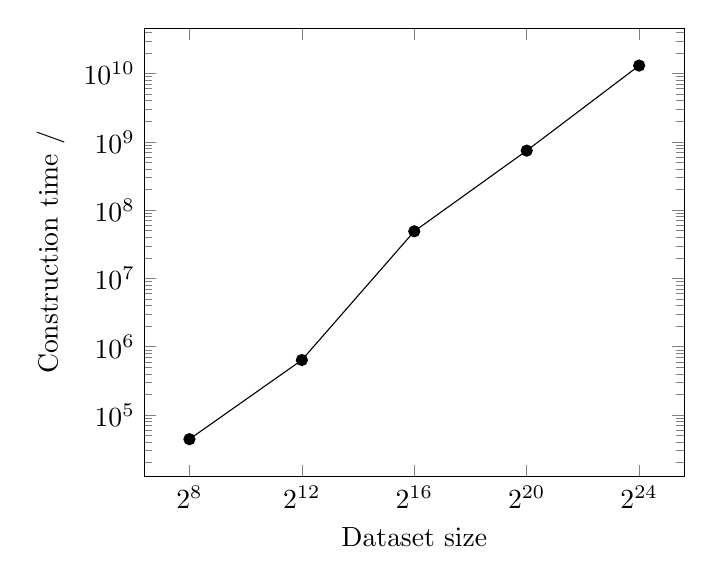
\begin{tikzpicture}
  \begin{loglogaxis}[
    log basis x = 2,
    log basis y = 10,
    xlabel = {Dataset size},
    xtick = {2^8, 2^12, 2^16, 2^20, 2^24},
    ylabel = {\text{Construction time} / \si{\nano\second}},
  ]
    \addplot [mark=*,black] coordinates {
      (256, 44277)
      (4096, 638777)
      (65536, 49027776)
      (1048576, 743982676)
      (16777216, 13091972575)
    };
  \end{loglogaxis}
\end{tikzpicture}
%
  \caption{Relationship between dataset size and summary construction time}
  \label{fig:fingerprint-implementation-performance}
\end{figure}

The results of all \num{25}~runs of each of the five performance tests are presented in \cref{tab:fingerprint-implementation-performance}, and the relationship between the size of a dataset and the time taken to construct its summary is shown in \cref{fig:fingerprint-implementation-performance}.
This relationship appears to be linear, which agrees with the analysis given in \cref{subsec:fingerprint-analysis-complexity}.
Since the update operation has constant amortized time complexity per update, and one update is performed for every item--weight pair in the dataset, the time complexity associated with performing all the updates given in a dataset is linear in the size of the dataset.
